\probheadernum{4}

% team 2.4

Consider 3 red balls and 5 blue balls arranged on a line from left to right. How many different orderings of balls are there on this line if each red ball must have a blue ball immediately to its right? Balls of the same color are indistinguishable.

\begin{enumerate}[(a)]
	\item  5

	\item  10

	\item  20

	\item  40

	\item  120

\end{enumerate}
\begin{solution}

B
\\
Each pair of (red, blue) becomes an entity (there are 3 of these). There are 2 remaining blue balls. The number of orderings of these 5 entities is $5!/(3! \cdot 2!)=120/(6 \cdot 2)=10$. Another way to view this problem is choosing where to put the 2 single blue balls among the 5 available spots, which is $\binom{5}{2} = 10$.

\end{solution}\probheadernum{4}

% team 3.2

What is the coefficient for the $m^{50} n^{51}$ term in the binomial expansion of $(3m-n)^{101}$
\begin{enumerate}[(a)]
	\item  $-(3^{51})\binom{101}{51}$ 
    
	\item  $-(3^{50})\binom{101}{50}$
    
	\item  $3^{50}\binom{101}{51}$ 
    
	\item  $3^{51}\binom{101}{50}$  

\end{enumerate}
\begin{solution}

B
\\
The binomial expansion is $\sum_{k=0}^{101}\binom{101}{k}(3m)^{k}(-n)^{101-k}$. Expanding this, we get $\sum_{k=0}^{101}(-1)^{101-k}3^{k}m^kn^{101-k}$. The term asked for is when $k = 50$, so plugging that into the coefficient, we get $\binom{101}{50}(-1)^{51}3^{50} = -(3^{50})\binom{101}{50}$. 

\end{solution}\probheadernum{4}

% team 3.3

How many ways are there to create an unordered group of 7 letters from the 26 English letters (lower-case only), where repetition is allowed?  
\begin{enumerate}[(a)]
	\item  \text{\Large{$\frac{26!}{7!7!7!7!7!7!7!}$}}
    
	\item  $\binom{26}{7}$
    
	\item  $\binom{32}{7}$
    
	\item  $\binom{33}{7}$
    
	\item  $P(26, 7)$

\end{enumerate}
\begin{solution}

C
\\
This is stars n' bars, with 7 stars and $26-1=25$ bars. There are $\binom{stars+bars}{stars} = \binom{7+25}{7}=\binom{32}{7}$ ways to create a group of 7 letters. You can also think about this problem as putting 7 indistinguishable objects in 26 distinguishable boxes.

\end{solution}\probheadernum{4}

% team 2.2

Consider a set $S$ that contains all integers between 1 and 203 inclusive. What is the minimum number of distinct integers you can pick from set $S$ such that you are guaranteed that at least 2 of those numbers sum to 204?\\

\begin{enumerate}[(a)]
	\item  2

	\item  101

	\item  102

	\item  103

	\item  202

\end{enumerate}
\begin{solution}

D

\end{solution}\probheadernum{4}

% team 3.5

We need to assign 4 students (A, B, C, and D) to 3 different teams (Team 1, Team 2, and Team 3). Each team needs to have at least 1 student. A and B cannot be in the same team. How many different ways are there to assign the teams?
\begin{enumerate}[(a)]
	\item  6  
    
	\item  24 
    
	\item  30
    
	\item  36

\end{enumerate}
\begin{solution}

C
\\
We need to put the 4 students into 3 groups and each group needs to have at least 1 student. This means two of the students need to be in the same team.  There are $C(4, 2)=6$ ways to select two students who will be on the same team. However, A and B cannot be in the same team, so there are $6-1=5$ ways to select the pair of students who will on the same team. We now have 3 groups of 1, 1, and 2 students, and we assign the 3 groups to 3 teams, so there are in total $5 \cdot P(3, 3)= 5 \cdot 3! = 30$ ways.


\end{solution}\probheadernum{4}

% team 1.2
Suppose we roll a fair die until we see a 2 and a 3 in no particular order. What is the expected value of the number of times we roll the die?

\begin{enumerate}[(a)]
	\item  6

	\item  9

	\item  12

	\item  18

	\item  24

\end{enumerate}
\begin{solution}

B
\\
Let X = number of rolls to get the first 2 or 3. $p=1/3$, so $E(X)=3$.\\
Let Y = number of rolls to get the other number. $p=1/6$, so $E(Y)=6$.\\
$E(X + Y) = E(X) + E(Y) = 3 + 6 = 9$.
%Let X = number of times we roll the dice get a 2 first and not 3 and then a 3, $E(X)= E(2) + E(3) = 3 + 6 = 9 $
%Let Y = number of times we roll the dice get a 3 first and not 2then a 2, $E(Y)= E(3) + E(2) = 3 + 6 = 9$
%total expected value
%\\ $E(X $ \cup $ Y) = E(X) + E(Y) = 18 $

\end{solution}\probheadernum{4}

% team 1.3

Consider a relation $R$ on the set of all sets, where two sets $A$ and $B$ are related via $R$ if and only if $A$ and $B$ have at least 3 elements in common. Which properties hold for this relation?

\begin{enumerate}[(a)]
	\item  Reflexive
    
	\item  Symmetric
    
	\item  Antisymmetric
    
	\item  Transitive

\end{enumerate}
\begin{solution}

B
\\
$R$ is not reflexive, because there is only 1 element in the intersection of a set of size 1 with
itself. $R$ is not antisymmetric; for example $\{1,2,3,4\}$ is related to $\{1,2,3\}$, but they are not the same set. $R$ is not transitive, because \{1, 2, 3, 4\} is related to \{1, 2, 3\} and \{2, 3, 4\} which are
not related, and $R$ is symmetric because $A \cap B$ = $B \cap A$.

\end{solution}\probheadernum{4}

% team 4.6

Two fair six-sided dice are rolled, where one is red and one is blue. Let $R$ be the event that the red die came up as a 3, and let $A$ be the event that at least one of the two dice came up as 3. Which of the following are true?

\begin{enumerate} [(a)]
    \item $P(A|R) = P(A)$
    \item $P(R|A) = P(R)$
    \item $P(A \cap R) = P(R)$
    \item $P(A) = \frac{1}{3}$
    \item $P(R) = \frac{1}{6}$
\end{enumerate}

\begin{solution}
C, E
\\
The intersection of "red die came up as a 3" and "at least one of the two dice came up as 3" should be still "red die came up as a 3", which means $P(A \cap R) = P(R)$. For (a), $P(A|R) = P(A \cap R)/P(R) = P(R)/P(R) = 1$. For (b), $P(R|A) = P(A \cap R)/P(A) = P(R)/P(A) \neq P(R)$. For (d), $P(A) = 11/36$ since there are 11 valid combinations out of 36(the size of sample space).
\end{solution}


\begin{enumerate}[(a)]
	\item  $P(A|R) = P(A)$
    
	\item  $P(R|A) = P(R)$
    
	\item  $P(A \cap R) = P(R)$
    
	\item  $P(A) = \frac{1}{3}$
    
	\item  $P(R) = \frac{1}{6}$

\end{enumerate}
\begin{solution}

C, E
\\
The intersection of "red die came up as a 3" and "at least one of the two dice came up as 3" should be still "red die came up as a 3", which means $P(A \cap R) = P(R)$. For (a), $P(A|R) = P(A \cap R)/P(R) = P(R)/P(R) = 1$. For (b), $P(R|A) = P(A \cap R)/P(A) = P(R)/P(A) \neq P(R)$. For (d), $P(A) = 11/36$ since there are 11 valid combinations out of 36(the size of sample space).

\end{solution}\probheadernum{4}

% team Misc.12

Now, there is a second bag with five balls numbered 1 through 5. Carol draws a ball from this second bag. Let $Z$ be the value of the ball Carol drew, and again let $X$ and $Y$ be values of the balls that Alice and Bob drew, respectively. Which of the following are true? 
\begin{enumerate} [(a)]
    \item $V(X) = \frac{2}{3}$
    \item $V(X+Y) = V(X)+V(Y)$
    \item $V(Z) = 2$
    \item $V(X+Z) = V(X)+V(Z)$
\end{enumerate}
\begin{solution}
A, C, D
\\
(B) is not guaranteed since $X$ and $Y$ are not independent. (D) works because $X$ and $Z$ are independent.
\end{solution}


\vspace{0.3in}
\begin{enumerate}[(a)]
	\item  $V(X) = \frac{2}{3}$
    
	\item  $V(X+Y) = V(X)+V(Y)$
    
	\item  $V(Z) = 2$
    
	\item  $V(X+Z) = V(X)+V(Z)$

\end{enumerate}
\begin{solution}

A, C, D
\\
(B) is not guaranteed since $X$ and $Y$ are not independent. (D) works because $X$ and $Z$ are independent.

\end{solution}\probheadernum{4}

% team 1.13

Suppose that $R$ and $S$ are relations on a set $A$. $R$ is reflexive and $S$ is symmetric. Which of the following statements must be true?

\begin{enumerate}[(a)]
	\item  $R \cup S$ is symmetric

	\item  $R \cap S$ is symmetric

	\item  $S - R$ is symmetric

	\item  $R^2$ is reflexive

\end{enumerate}
\begin{solution}

D

\end{solution}\probheadernum{4}
\\
title page question
\begin{enumerate}[(a)]
\end{enumerate}
\begin{solution}
uestion

\end{solution}\probheadernum{4}
\\
% Team 2, Question 5
\textit{Reminders:} A standard deck has 52 cards with 4 suits ($\heartsuit, \diamondsuit, \clubsuit, \spadesuit$) and 13 ranks (2, 3, \dots, 10, Jack (J), Queen (Q), King (K), Ace (A)). \\

Joseph randomly draws a hand of $13$ cards from a standard deck of cards. What is the probability of his hand contains exactly two Aces?
\begin{enumerate}[(a)]
	\item  $\frac{4\cdot3\cdot\binom{48}{11}}{\binom{52}{13}}$

	\item  $\frac{\binom{4}{2}\cdot\binom{48}{11}}{\binom{52}{13}}$

	\item  $\left(\frac{4}{52}\right)^2\cdot\left(\frac{48}{52}\right)^{11}$

	\item  $\left(\frac{4}{52}\right)^2\cdot\left(\frac{48}{52}\right)^{11}\cdot(13)!$

	\item  $\left(\frac{4}{52}\right)^2\cdot\left(\frac{48}{52}\right)^{11}\cdot\binom{13}{2}$

\end{enumerate}
\begin{solution}

(b)\\
The size of the sample space is the number of ways to choose $13$ cards out of $52$ cards, which is $\binom{52}{13}$. The task of drawing $13$ cards with exactly two Aces can be viewed as the cascade of drawing $2$ Aces out of $4$ Aces and drawing $11$ non-Aces out of $48$ non-Aces. By the product rule, the size of the event is $\binom{4}{2}\cdot\binom{48}{11}$. Since we assume random drawing, all outcomes in the sample space are equally likely, the probability is $\frac{\binom{4}{2}\cdot\binom{48}{11}}{\binom{52}{13}}$.

\end{solution}\probheadernum{4}
\\
% Team 3, Question 1
Brian dealt out a standard 52-card deck of cards. What is the probability that the first King occurs on the 20th card?
\begin{enumerate}[(a)]
	\item  $\frac{\binom{52}{19}\cdot\binom{4}{1}\cdot42!}{52!}$

	\item  $\frac{(48!/29!)\cdot32!\cdot4}{52!}$

	\item  $\frac{51!\cdot4}{52!}$

	\item  $\frac{(48!/29!)\cdot4}{52!}$

	\item  $(\frac{48}{52})^{19}\cdot\frac{4}{52}$

\end{enumerate}
\begin{solution}

(b)\\
The sample space is all the possible permutations of 52 cards. The event is the set of permutations that the first king occurs at the 20th position. The first 19 positions must not have rank of king, and hence $\frac{48!}{29!}$ ways to form the first 19 positions. 4 options at the 20th position because each rank can take on 4 possible suits. The arrangement of the rest of 32 cards has no constraint, and there are 32! ways to form the remaining 32 positions.

\end{solution}\probheadernum{4}
\\
% Greg, Binomial Coefficient Question
In the binomial expansion of $(1/x^2 + x)^{15}$, what is the coefficient of the term $x^7$?
\begin{enumerate}[(a)]
	\item  0
    
	\item  $15 \choose 7$
    
	\item  $15 \choose 5$
    
	\item  $15 \choose 9$
    
	\item  1

\end{enumerate}
\begin{solution}

(a)\\
Expand the expression
\begin{align*}
(x^{-2} + x)^{15}  =& \sum_{k=0}^{15} {15\choose k}{(x^{-2})}^k {x}^{15-k} \\
=& \sum_{k=0}^{15} {15\choose k}x^{-2k} x^{15-k} \\
=& \sum_{k=0}^{15} {15\choose k}x^{-2k+15-k} \\
=& \sum_{k=0}^{15} {15\choose k}x^{15-3k}\\
\end{align*}
Since the non-zero terms in the expansion have exponents that are multiples of 3, the coefficient for $x^7$ is 0. 

\end{solution}\probheadernum{4}
\\
% Team 2, Question 3
How many 52 letter non-decreasing strings are there when the letters are chosen with repetition from the 26-letter English alphabet (abcdefghijklmnopqrstuvwxyz)?\\
(Note: Non-decreasing means that a letter at a latter position can only be the same or greater than its former letter, so a string of ``aabxzzzz" would be valid, whereas ``a\textbf{\underline{db}}" would not be valid.)\\
\textit{Hint:} Consider how you can use stars and bars to solve this.
\begin{enumerate}[(a)]
	\item  $\binom{52}{26}$

	\item  $\binom{77}{51}$

	\item  $26^{52}$

	\item  $\binom{77}{25}$

	\item  $\binom{78}{51}$

\end{enumerate}
\begin{solution}

(d)\\
This boils down to a Stars and Bars problem. We just need to choose the letters of the string, since once we have letters there is exactly one way to make a valid string (arrange the letters in a non-decreasing order). We have 25 bars coming from the 26 possible letter choices. Each letter in the string is a star that fits into one of the letter boxes. We have $\binom{\text{stars+bars}}{\text{stars}}=\binom{25+52}{25}=\binom{77}{25}$ possible strings.

\end{solution}\probheadernum{4}
\\
% Team 2, Question 6
Which of the following represent the number of strings that consist of exactly 5 A's, 4 B's, and 3 C's?  Select all that apply.
\begin{enumerate}[(a)]
	\item  $3^{12}$

	\item  $\binom{12}{5}\cdot\binom{12}{4}\cdot\binom{12}{3}$

	\item  $\frac{12!}{5!\cdot4!\cdot3!}$

	\item  $\binom{12}{5}\cdot\binom{7}{4}\cdot\binom{3}{3}$

	\item  $5!\cdot 4!\cdot 3!$

\end{enumerate}
\begin{solution}

(c),(d)
\begin{enumerate}[(a)]
\addtocounter{enumi}{2}
\item counts all permutations of 12 possible letters, then divides by repeated letters to avoid overcounting. 
\item computes multinomial coefficients by choosing where all repetitions of a given letter go at once $\binom{12}{5}\cdot \binom{7}{4}\cdot\binom{3}{3}$.
\end{enumerate}

\end{solution}\probheadernum{4}


There are 50 participants in a TV show. The host of the show will distribute three identical prizes among the participants by spinning a wheel that has numbers 1 through 50 on it three times. How many ways are there to distribute the prizes?

\begin{enumerate}[(a)]
	\item  $\frac{50^3}{3!}$
    
	\item  $50^3$
    
	\item  $\binom{52}{2}$
    
	\item  $\binom{52}{49}$
    
	\item  $\binom{50}{3}$

\end{enumerate}
\begin{solution}

(d) \\
Note that any individual can win anywhere between 0 and 3 prizes, inclusive (repetition). By stars n' bars, we see that there are 3 stars and 49 bars. Since the prizes are identical (indistinguishable) then we treat the prizes as stars, and the participants are distinguishable and are used to calculate bars as $50 - 1 = 49$. Thus, there are $\binom{52}{3} = \binom{52}{49}$ ways to award the prizes.

\end{solution}\probheadernum{4}


Grace has 3 red balls, 3 blue balls, and 4 green balls. She wants to put the balls into $x$ boxes that can each hold any number of balls. What's the largest value of $x$ such that Grace can guarantee that at least two of the same colored balls are in some box? 

\begin{enumerate}[a)]
\item 3
\item 4
\item 7
\item 9
\item 10
\end{enumerate}

\begin{solution}
(a) \\
This is because for red balls and blue balls, it's possible that they are distributed evenly among the three boxes. However, for green balls, there are 4 balls but only 3 boxes, so using the pigeonhole principle, $\lceil \frac{4}{3} \rceil = 2$. \\
For any value of $ x > 3$ (ex. 4), we can't apply pigeonhole principle because the number of boxes are greater or equal to the number of balls of each color.
\end{solution}

\newpage
%\vspace{2cm}
\begin{enumerate}[(a)]
	\item  3

	\item  4

	\item  7

	\item  9

	\item  10

\end{enumerate}
\begin{solution}

(a) \\
This is because for red balls and blue balls, it's possible that they are distributed evenly among the three boxes. However, for green balls, there are 4 balls but only 3 boxes, so using the pigeonhole principle, $\lceil \frac{4}{3} \rceil = 2$. \\
For any value of $ x > 3$ (ex. 4), we can't apply pigeonhole principle because the number of boxes are greater or equal to the number of balls of each color.

\end{solution}\probheadernum{4}


What is the big-$\Theta$ runtime of this algorithm when the input is a positive integer $n$?

\begin{algorithm}[H]
    \SetKwFunction{Alg}{Alg}{}
    \SetKwFunction{Print}{print}
    \SetKwProg{Fn}{procedure}{\string:}{}
    \SetKwFor{For}{for}{do}{}
    \SetKwFor{While}{while}{do}{}
    \SetKwInOut{Input}{input}
    \DontPrintSemicolon
    \Input{$n$, a positive integer}
    \BlankLine
    \Fn{\Alg{n}}{
        $k=1$ \\
        \For{$i := 1$ \KwTo $n$}{
            $k=k * 2$
         }
         \While{$(k>1)$} {
            $k = k / 10$
         }
         \KwRet{}
     }
     \caption{Alg}
\end{algorithm}

\begin{enumerate}[a)]
\item $\Theta(\log n)$
\item $\Theta(n)$
\item $\Theta(n^2)$
\item $\Theta(2^n)$
\item $\Theta(2^n \log n)$
\end{enumerate}

\begin{solution}
(b) \\
The first for loop iterates $n$ times and the value of $k$ becomes $2^n$. \\
The while loop iterates $\log_{10} k = \log_{10} (2^n) = n \log_{10} 2$ times, where $\log_{10} 2$ is a constant. \\
Therefore, this algorithm runs in $\Theta(n)$ time.
\end{solution}

\newpage
\begin{enumerate}[(a)]
	\item  $\Theta(\log n)$

	\item  $\Theta(n)$

	\item  $\Theta(n^2)$

	\item  $\Theta(2^n)$

	\item  $\Theta(2^n \log n)$

\end{enumerate}
\begin{solution}

(b) \\
The first for loop iterates $n$ times and the value of $k$ becomes $2^n$. \\
The while loop iterates $\log_{10} k = \log_{10} (2^n) = n \log_{10} 2$ times, where $\log_{10} 2$ is a constant. \\
Therefore, this algorithm runs in $\Theta(n)$ time.

\end{solution}\probheadernum{4}


Suppose you randomly select an integer from the set $\{1, 2, \dots, 1000\}$. What is the expected number of digits in the selected number?

\begin{enumerate}[a)]
    \item 2.888
    \item 2.893
    \item 3.21
    \item 3.228
    \item None of the above
\end{enumerate}

\begin{solution}
(b) \\
Let X represent the number of digits in the selected number. X could take on the value 1, 2, 3, or 4 since there could be anywhere between 1 to 4 digits in the selected number. Now to find $E(X)$, we have to determine the probability that X takes on each of 1, 2, 3, or 4. We do this by calculating $\frac{|E|}{|S|}$, with $|S| = 1000$ since there are $1000$ numbers in our sample space.\\
\newline
$P(X = 1) = \frac{|\{1, 2, \dots, 9\}|}{1000} = \frac{9}{1000}$.\\
$P(X = 2) = \frac{|\{10, 11, \dots, 99\}|}{1000} = \frac{90}{1000}$.\\
$P(X = 3) = \frac{|\{100, 101, \dots, 999\}|}{1000} = \frac{900}{1000}$.\\
$P(X = 4) = \frac{|\{1000\}|}{1000} = \frac{1}{1000}$.\\
\newline
    $E(X) = 1 (\frac{9}{1000}) + 2 (\frac{90}{1000}) + 3 (\frac{900}{1000}) + 4 (\frac{1}{1000}) = \frac{9 + 180 + 2700 + 4}{1000} = 2.893$

\end{solution}

%\vspace{.6cm}
\newpage
\begin{enumerate}[(a)]
	\item  2.888
    
	\item  2.893
    
	\item  3.21
    
	\item  3.228
    
	\item  None of the above

\end{enumerate}
\begin{solution}

(b) \\
Let X represent the number of digits in the selected number. X could take on the value 1, 2, 3, or 4 since there could be anywhere between 1 to 4 digits in the selected number. Now to find $E(X)$, we have to determine the probability that X takes on each of 1, 2, 3, or 4. We do this by calculating $\frac{|E|}{|S|}$, with $|S| = 1000$ since there are $1000$ numbers in our sample space.\\
\newline
$P(X = 1) = \frac{|\{1, 2, \dots, 9\}|}{1000} = \frac{9}{1000}$.\\
$P(X = 2) = \frac{|\{10, 11, \dots, 99\}|}{1000} = \frac{90}{1000}$.\\
$P(X = 3) = \frac{|\{100, 101, \dots, 999\}|}{1000} = \frac{900}{1000}$.\\
$P(X = 4) = \frac{|\{1000\}|}{1000} = \frac{1}{1000}$.\\
\newline
    $E(X) = 1 (\frac{9}{1000}) + 2 (\frac{90}{1000}) + 3 (\frac{900}{1000}) + 4 (\frac{1}{1000}) = \frac{9 + 180 + 2700 + 4}{1000} = 2.893$


\end{solution}\probheadernum{4}


What is the coefficient for the $y^{25}$ term in the expansion of $((3x^2+\frac{5}{x^3})y)^{25}$? \\
Note: There are no typos in this question.

\begin{enumerate}[(a)]
	\item  0

	\item  $\binom{25}{13}3^{12}\cdot 5^{13}$

	\item  $\binom{25}{25}3^{0}\cdot 5^{25}$

	\item  $\binom{25}{15}3^{15}\cdot 5^{10}$

	\item  $\binom{25}{5}3^{20}\cdot 5^{5}$

\end{enumerate}
\begin{solution}

(d) \\
We can write $((3x^2+\frac{5}{x^3})y)^{25}=(3x^2y+\frac{5y}{x^3})^{25}$. When the first term is raised to the 15th power and the second term is raised to the 10th power, the $x$ term disappears and we are left with $y^{25}$. Thus, the coefficient is $\binom{25}{10}3^{15}\cdot 5^{10}=\binom{25}{15}3^{15}\cdot 5^{10}$

\end{solution}\probheadernum{4}


Let $R$ be a relation over the set of all sets. For sets $A$ and $B$, let ${}_A R_B$ if and only if $A - B$ is finite. Which of the following are true about $R$?
\begin{enumerate}[a)]
    \item reflexive
    \item symmetric
    \item antisymmetric
    \item transitive
\end{enumerate}
\begin{solution}
(a), (d)\\
\begin{enumerate}[a)]
    \item True; For every set $A$, $A - A = \emptyset$ and since the empty set is finite, then R is reflexive.
    \item False; Choose $A = \mathbb{Z^+}$ and $B = \mathbb{Z}$. Then ${}_A R_B$ because $A - B = \emptyset$, but $\neg {}_B R_A$ because $B - A = \mathbb{Z^-} \cup \{0\}$ which is countable infinite (not finite).
    \item False; Choose $A = \{1\}$ and $B = \{2\}$. Then ${}_A R_B$ because $A - B = \{1\}$ which is finite and ${}_B R_A$ because $B - A = \{2\}$ which is finite, but $A \neq B$.
    \item True; For arbitrary sets $A, B, C$, suppose that ${}_A R_B$ and ${}_B R_C$. We would like to show that ${}_A R_C$. Since ${}_A R_B$ then $A - B = A \cap \overline{B}$ is finite and since ${}_B R_C$ then $B - C = B \cap \overline{C}$ is finite. Then because the union of 2 finite sets must also be finite, we investigate and simplify $(A \cap \overline{B}) \cup (B \cap \overline{C}) = (A \cup B) \cap (A \cup \overline{C}) \cap (\overline{B} \cup \overline{C})$.\\
    If ${}_A R_C$, it would have to be true that $A - C = A \cap \overline{C}$ is finite. This can be proven by showing that $A \cap \overline{C} \subseteq (A \cup B) \cap (A \cup \overline{C}) \cap (\overline{B} \cup \overline{C})$. For any arbitrary $x \in A \cap \overline{C}$, $x \in A$ and $x \in \overline{C}$ by definition of set intersection. Since $x \in A$, then we know $x \in A$ or $x \in B$, so $x \in A \cup B$ and we know $x \in A$ or $x \in \overline{C}$, so $x \in A \cup \overline{C}$ by definition of set union. Also, since $x \in \overline{C}$, then we know $x \in \overline{B}$ or $x \in \overline{C}$, so $x \in \overline{B} \cup \overline{C}$. Thus, $x \in (A \cup B) \cap (A \cup \overline{C}) \cap (\overline{B} \cup \overline{C})$, so $A \cap \overline{C} \subseteq (A \cup B) \cap (A \cup \overline{C}) \cap (\overline{B} \cup \overline{C})$. Therefore, $A \cap \overline{C} = A - C$ must be finite, so ${}_A R_C$, which proves that R must be transitive.
\end{enumerate}
\end{solution}

\vspace{2cm}
\begin{enumerate}[(a)]
	\item  reflexive
    
	\item  symmetric
    
	\item  antisymmetric
    
	\item  transitive

\end{enumerate}
\begin{solution}

(a), (d)\\
\begin{enumerate}[a)]
    \item True; For every set $A$, $A - A = \emptyset$ and since the empty set is finite, then R is reflexive.
    \item False; Choose $A = \mathbb{Z^+}$ and $B = \mathbb{Z}$. Then ${}_A R_B$ because $A - B = \emptyset$, but $\neg {}_B R_A$ because $B - A = \mathbb{Z^-} \cup \{0\}$ which is countable infinite (not finite).
    \item False; Choose $A = \{1\}$ and $B = \{2\}$. Then ${}_A R_B$ because $A - B = \{1\}$ which is finite and ${}_B R_A$ because $B - A = \{2\}$ which is finite, but $A \neq B$.
    \item True; For arbitrary sets $A, B, C$, suppose that ${}_A R_B$ and ${}_B R_C$. We would like to show that ${}_A R_C$. Since ${}_A R_B$ then $A - B = A \cap \overline{B}$ is finite and since ${}_B R_C$ then $B - C = B \cap \overline{C}$ is finite. Then because the union of 2 finite sets must also be finite, we investigate and simplify $(A \cap \overline{B}) \cup (B \cap \overline{C}) = (A \cup B) \cap (A \cup \overline{C}) \cap (\overline{B} \cup \overline{C})$.\\
    If ${}_A R_C$, it would have to be true that $A - C = A \cap \overline{C}$ is finite. This can be proven by showing that $A \cap \overline{C} \subseteq (A \cup B) \cap (A \cup \overline{C}) \cap (\overline{B} \cup \overline{C})$. For any arbitrary $x \in A \cap \overline{C}$, $x \in A$ and $x \in \overline{C}$ by definition of set intersection. Since $x \in A$, then we know $x \in A$ or $x \in B$, so $x \in A \cup B$ and we know $x \in A$ or $x \in \overline{C}$, so $x \in A \cup \overline{C}$ by definition of set union. Also, since $x \in \overline{C}$, then we know $x \in \overline{B}$ or $x \in \overline{C}$, so $x \in \overline{B} \cup \overline{C}$. Thus, $x \in (A \cup B) \cap (A \cup \overline{C}) \cap (\overline{B} \cup \overline{C})$, so $A \cap \overline{C} \subseteq (A \cup B) \cap (A \cup \overline{C}) \cap (\overline{B} \cup \overline{C})$. Therefore, $A \cap \overline{C} = A - C$ must be finite, so ${}_A R_C$, which proves that R must be transitive.
\end{enumerate}

\end{solution}\probheadernum{4}


Which of the following are true?

\begin{enumerate}[a)]
    \item $(n^2 + 5n^4 - 7)(6 - n)$ is $\Theta (n^4)$
    \item $(n^3 + \frac{5}{n})^{15}$ is $O(n^{30})$
    \item $3^n + n^3 + 3!$ is $O(4^n)$
    \item $\sum\limits_{k=0}^{20} n \cdot 3^k$ is $\Theta(n)$
    \item $n^n$ is $O(n!)$
\end{enumerate}

\begin{solution}
(c), (d)\\
\begin{enumerate}[a)]
    \item False; Looking at the highest-degree term from each factor, this expression would be $\Theta (n^4 \cdot n) = \Theta (n^5)$ which is not $\Theta (n^4)$.
    \item False; This expression will have as large as an $n^{45}$ term which is larger than $n^{30}$, therefore it is not $O(n^{30})$.
    \item True; $3^n + n^3 + 3!$ is $O(3^n)$ which is also $O(4^n)$ since $4^n$ grows faster than $3^n$.
    \item True; $\sum\limits_{k=0}^{20} n \cdot 3^k = n \cdot \sum\limits_{k=0}^{20} 3^k$ since the $n$ term does not at all depend on the bounds $k$. Then since $\sum\limits_{k=0}^{20} 3^k$ is just a constant, then the whole expression is $\Theta(n)$.
    \item False; Suppose there exists a $C \in \mathbb{R}$ such that $n^n \leq C \cdot n!$ for all $n \geq k \in \mathbb{R}$.
    \begin{align*}
        n^n &\leq C \cdot n!\\
        n \cdot n \cdot n \dots \cdot n &\leq C \cdot n \cdot (n - 1) \cdot (n - 2) \dots \cdot 1\\
        \frac{n}{n} \cdot \frac{n}{n - 1} \cdot \frac{n}{n - 2} \dots \cdot \frac{n}{1} &\leq C\\
        C &\geq \frac{n}{n} \cdot \frac{n}{n - 1} \cdot \frac{n}{n - 2} \dots \cdot \frac{n}{1} \geq n\\
    \end{align*}
    Therefore, for any choice of $C$, we can choose an $n > C$, say $C +1$ to disprove our assumption. Therefore, $n^n$ is not $O(n!)$.
\end{enumerate}
\end{solution}

\newpage
\begin{enumerate}[(a)]
	\item  $(n^2 + 5n^4 - 7)(6 - n)$ is $\Theta (n^4)$
    
	\item  $(n^3 + \frac{5}{n})^{15}$ is $O(n^{30})$
    
	\item  $3^n + n^3 + 3!$ is $O(4^n)$
    
	\item  $\sum\limits_{k=0}^{20} n \cdot 3^k$ is $\Theta(n)$
    
	\item  $n^n$ is $O(n!)$

\end{enumerate}
\begin{solution}

(c), (d)\\
\begin{enumerate}[a)]
    \item False; Looking at the highest-degree term from each factor, this expression would be $\Theta (n^4 \cdot n) = \Theta (n^5)$ which is not $\Theta (n^4)$.
    \item False; This expression will have as large as an $n^{45}$ term which is larger than $n^{30}$, therefore it is not $O(n^{30})$.
    \item True; $3^n + n^3 + 3!$ is $O(3^n)$ which is also $O(4^n)$ since $4^n$ grows faster than $3^n$.
    \item True; $\sum\limits_{k=0}^{20} n \cdot 3^k = n \cdot \sum\limits_{k=0}^{20} 3^k$ since the $n$ term does not at all depend on the bounds $k$. Then since $\sum\limits_{k=0}^{20} 3^k$ is just a constant, then the whole expression is $\Theta(n)$.
    \item False; Suppose there exists a $C \in \mathbb{R}$ such that $n^n \leq C \cdot n!$ for all $n \geq k \in \mathbb{R}$.
    \begin{align*}
        n^n &\leq C \cdot n!\\
        n \cdot n \cdot n \dots \cdot n &\leq C \cdot n \cdot (n - 1) \cdot (n - 2) \dots \cdot 1\\
        \frac{n}{n} \cdot \frac{n}{n - 1} \cdot \frac{n}{n - 2} \dots \cdot \frac{n}{1} &\leq C\\
        C &\geq \frac{n}{n} \cdot \frac{n}{n - 1} \cdot \frac{n}{n - 2} \dots \cdot \frac{n}{1} \geq n\\
    \end{align*}
    Therefore, for any choice of $C$, we can choose an $n > C$, say $C +1$ to disprove our assumption. Therefore, $n^n$ is not $O(n!)$.
\end{enumerate}

\end{solution}\probheadernum{4}


\emph{Reminders}: A standard deck has 52 cards, with 4 suits ($\heartsuit, \diamondsuit, \clubsuit, \spadesuit
$) and 13 ranks (2, 3, \dots, 10, J, Q, K, A).\\

\noindent
How many different 8-card poker hands have 3 cards that share a rank, 3 cards that share a different rank, and 2 cards that share another rank? For example, your hand may contain $2\heartsuit, 2\diamondsuit, 2\clubsuit, 5\spadesuit, 5\diamondsuit, 5\heartsuit,\text{J}\spadesuit,\text{J}\heartsuit$.

\begin{enumerate}[(a)]
	\item  $\binom{13}{3}\cdot 3\cdot 4\cdot 4\cdot 6{}$

	\item  $\frac{13\cdot 12\cdot 11\cdot\binom{4}{3}\binom{4}{3}\binom{4}{2}}{6}$

	\item  $\frac{52\cdot 3\cdot 2\cdot 48\cdot 3\cdot 2\cdot 44\cdot 3}{6\cdot 6\cdot 2\cdot 2}$

	\item  $\binom{13}{2}\binom{11}{1}\binom{4}{2}4^2$

	\item  $13\cdot 12\cdot 44 \cdot 3\cdot 4\cdot 4$

\end{enumerate}
\begin{solution}

(a) (c) (d)
\begin{enumerate}[(a)]
\item This is first choosing all the ranks then picking 1 of the 3 as the rank of the 2 cards of the same rank. Then we have 4 ways to choose one suit to not be in the hand for each of the groups of 3 cards that share a rank. And similarly for the other rank. Then $\binom{4}{2}=6$ ways to choose the 2 suits for the 2 cards of a rank.
\item This divides out too much. The only overcounting occurs with the $13\cdot 12$, thus we would only have to divide out 2 and not 6.
\item This is just picking all the cards separately then dividing out all the overcounting, we must divide by 6 twice then 2 twice, as the first 3 cards can be selected in any order and then the order of the ranks for the first 6 cards can be reversed (a divide by 2). Then again the order of the last 2 cards can be reversed, thus we must again divide by 2 there.
\item This is just picking 2 ranks for the groups 3 cards that share a rank, then picking a rank for the 2 cards that share a rank, then picking 2 suits for the 2 cards that share a rank and $\binom{4}{3}=4$ ways to pick 3 suits for each of the two remaining ranks.
\item This is picking a rank for the 3 cards that share a rank, then picking another rank for the 3 cards that share a rank. We are overcounting, because the order doesn't matter, thus we must divide out by 2. Then from the remaining 44 cards, picking a card then picking another card of the same rank. Again we are overcounting and must divide out by 2, because the order we select the cards doesn't matter. After we have 4 choices to select the one card of the rank that is not in our hand. This occurs two times (once for each rank of 3 cards of a kind). Thus the $2\cdot 2$ is never divided out, so we are overcounting.
\end{enumerate}

\end{solution}\probheadernum{4}


Which of the following are true about graphs?

\begin{enumerate}[a)]
    \item $K_5$ is bipartite
    \item $C_{60}$ is bipartite
    \item It is possible to have 56 edges in a bipartite graph with 14 vertices
    \item $Q_4$ has more vertices than $W_8$
    \item All directed multigraphs with $n$ vertices have more edges than all simple graphs with $n$ vertices 
\end{enumerate}

\begin{solution}
(b), (d)\\
\begin{enumerate}[a)]
    \item False; $K_5$ is not bipartite since $K_5$ contains triangles which are cycles of odd length and any time a graph contains a cycle of odd length, the graph cannot be bipartite.
    \item True; $C_{60}$ is bipartite because $60$ is even and any $C_{n}$ with even $n$ is bipartite by assigning one vertex a color and then alternating colors at every vertex along the cycle.
    \item False; The maximum possible edges in a bipartite graph with $2n$ vertices is $n^2$. This is because we must partition our set of vertices into two sets where no vertices within the same set are connected by an edge. When this is true, we maximize the number of edges by having every edge possible between vertices in separate sets. So if $k$ is the number of vertices in one partition, then $2n - k$ is the number in the other partition, creating a maximum of $k(2n - k)$ edges. This product is maximized when $k = n$, producing $n^2$ edges at maximum. Therefore, if we have 14 vertices in a bipartite graph, then we have a maximum of 49 edges.
    \item True; $Q_4$ has $2^4 = 16$ vertices, whereas $W_8$ only has $8 + 1 = 9$ vertices.
    \item False; A directed multigraph with $n$ vertices \textit{might} have more edges than a simple graph with $n$ vertices but it also might not. For example, let $G_1 = K_4$. $G_1$ is simple graph with 4 vertices and $\binom{4}{2} = 6$ edges. Now let $G_2$ be a directed multigraph with 4 vertices and 0 edges. Then $G_1$ and $G_2$ have the same number of vertices, but $G_1$ has more edges than $G_2$.
\end{enumerate}
\end{solution}

\newpage
\begin{enumerate}[(a)]
	\item  $K_5$ is bipartite
    
	\item  $C_{60}$ is bipartite
    
	\item  It is possible to have 56 edges in a bipartite graph with 14 vertices
    
	\item  $Q_4$ has more vertices than $W_8$
    
	\item  All directed multigraphs with $n$ vertices have more edges than all simple graphs with $n$ vertices 

\end{enumerate}
\begin{solution}

(b), (d)\\
\begin{enumerate}[a)]
    \item False; $K_5$ is not bipartite since $K_5$ contains triangles which are cycles of odd length and any time a graph contains a cycle of odd length, the graph cannot be bipartite.
    \item True; $C_{60}$ is bipartite because $60$ is even and any $C_{n}$ with even $n$ is bipartite by assigning one vertex a color and then alternating colors at every vertex along the cycle.
    \item False; The maximum possible edges in a bipartite graph with $2n$ vertices is $n^2$. This is because we must partition our set of vertices into two sets where no vertices within the same set are connected by an edge. When this is true, we maximize the number of edges by having every edge possible between vertices in separate sets. So if $k$ is the number of vertices in one partition, then $2n - k$ is the number in the other partition, creating a maximum of $k(2n - k)$ edges. This product is maximized when $k = n$, producing $n^2$ edges at maximum. Therefore, if we have 14 vertices in a bipartite graph, then we have a maximum of 49 edges.
    \item True; $Q_4$ has $2^4 = 16$ vertices, whereas $W_8$ only has $8 + 1 = 9$ vertices.
    \item False; A directed multigraph with $n$ vertices \textit{might} have more edges than a simple graph with $n$ vertices but it also might not. For example, let $G_1 = K_4$. $G_1$ is simple graph with 4 vertices and $\binom{4}{2} = 6$ edges. Now let $G_2$ be a directed multigraph with 4 vertices and 0 edges. Then $G_1$ and $G_2$ have the same number of vertices, but $G_1$ has more edges than $G_2$.
\end{enumerate}

\end{solution}\probheadernum{4}


How many ways are there to pair up 6 dogs with 6 different dog leashes, where each pair consists of a dog with a leash?

\begin{enumerate}[(a)]
	\item  6!

	\item  $2^6$

	\item  $(6!)^2$

	\item  $\binom{6+5}{6}$

	\item  $\binom{12}{2}\binom{10}{2}\binom{8}{2}\binom{6}{2}\binom{4}{2}$

\end{enumerate}
\begin{solution}

(a) \\
This is essentially assigning every dog a leash. The first dog can have 6 choices for a leash to pair with, the second dog has 5 choices and so on. Thus we have $6\cdot 5\cdot 4\cdot 3\cdot 2\cdot 1=6!$

\end{solution}\probheadernum{4}


What is the big-$\Theta$ of the following algorithm, based on the number of print statements?

% See: http://mirror.hmc.edu/ctan/macros/latex/contrib/algorithm2e/doc/algorithm2e.pdf
\begin{algorithm}[H]
    \SetKwFunction{Cheering}{Cheering}{}
    \SetKwFunction{Print}{print}
    \SetKwProg{Fn}{procedure}{\string:}{}
    \SetKwFor{For}{for}{do}{}
    \SetKwFor{If}{if}{then}{}
    \SetKwInOut{Input}{input}
    \DontPrintSemicolon
    \Input{$n$ an integer power of 2}
    \BlankLine
    \Fn{\Cheering{n}}{
        \If {$n = 1$} {
            \KwRet{}
        }
        \Cheering{$n/2$}\;
        \For{$i\leftarrow 1$ \KwTo $5$}{
            \For{$j\leftarrow 1$ \KwTo $n$}{
                \Print{``you got this!''}
            }
         }
         \Cheering{$n/2$}\;
         \Cheering{$n/2$}\;
         \KwRet{}
     }
     \caption{Cheering}
\end{algorithm}

\begin{enumerate}[(a)]
	\item  $\Theta(n)$

	\item  $\Theta(n^2)$

	\item  $\Theta(n^2\log(n))$

	\item  $\Theta(n \log(n^2))$

	\item  $\Theta(n^{\log_2 3})$

\end{enumerate}
\begin{solution}

% Hw Team 4
(e)\\
$Cheering$ calls itself 3 times, each with an input size of $n/2$. Outside of the recursive calls, $Cheering$ executes the print statement inside the nested for loops. The inner loop executes $n$ times for each index of the outer loop, and the outer loop executes 5 times, so \textit{``you got this!"} is printed $5n$ times.
Putting it all together, the complexity of the algorithm, based on the number of print statements, is:
$T(n) = 3T(n/2) + 5n$.\\

 Using the Master Theorem, we can see that $a = 3, b = 2, d = 1$, so $\frac{a}{b^d} = 3/2 > 1$. Therefore, the complexity of this function is $=\Theta(n^{\log_b a})= \Theta(n^{\log_2 3})$

\end{solution}\probheadernum{4}


Let A be a set such that $|A| = 5$. How many relations over $A$ are reflexive? 

\begin{enumerate}[(a)]
	\item  5
    
	\item  $2^{25} - 5 \cdot 2^{24}$
    
	\item  $\sum\limits_{k=1}^{20} \binom{25}{k}$ 
    
	\item  $2^{11}$
    
	\item  $2^{20}$

\end{enumerate}
\begin{solution}

% HW TEAM 2
(e) \\
Of the $5^2 = 25$ potential  edges between elements of $A$, we know that 5 must be in the relation since our relation must be reflexive. That is, of the 25 possible ordered pairs that could be in the relation, we know that all 5 pairs of the form $(x,x)$ must be in the relation in order for it to be reflexive. For the remaining 20 potential ordered pairs, each pair could either be in the relation or not in the relation, giving  $2^{20}$ possible relations.

\end{solution}\probheadernum{4}


Which of the following values of $x$ satisfy the congruence $3x \equiv 10$ (mod 12)?
\begin{enumerate}[(a)]
	\item  4

	\item  10

	\item  12

	\item  20

	\item  22

\end{enumerate}
\begin{solution}

%TEAM 1
None of the above. $3x \equiv 10$ (mod 12) has no solutions. The only possible values of $3x$ in (mod 12) are \{0,3,6,9\}, thus $3x$ can never be 10.

\end{solution}\probheadernum{4}


Which of the following are true?

\begin{enumerate}[(a)]
	\item  gcd$(108,25) = 1$

	\item  $25x \equiv 29 \pmod{108}$ has a solution.

	\item  $25^{-1} \equiv -4$  (mod  108)

	\item  $25^{-1} \equiv 13$  (mod 108)

	\item  $25^{-1}$ does not exist  (mod $108$)

\end{enumerate}
\begin{solution}
 a, b, d
% Hw team 1

We can implement the Extended Euclidean Algorithm on (108, 25) to answer all parts of this problem.
    \begin{align*}
        108-4\cdot 25 &=8 &\\
        25 -3 \cdot 8 &= 1 & \text{so} \gcd(108,25)=1\\
        \text{Working back up: }\\
        1&= 25-3\cdot 8 \\
         &= 25 - 3(108 - 4 \cdot 25) \\
         &= -3\cdot 108 +13 \cdot 25 \\
    \end{align*}
    

Looking at $1= -3\cdot 108 +13 \cdot 25$ in (mod 108), we get $1 \equiv 13 \cdot 25$ (mod 108) from which we observe that 13 and 25 are inverses in (mod 108). 

\end{solution}\probheadernum{4}


Given the poset $(\{-3, 1, 2,  5, 12, 9, 36\}, |)$, which of the following statements are true?

\begin{enumerate}[(a)]
	\item  
    There is at least one maximum element.
    
	\item 
    There is at least one minimum element.
    
	\item 
    There is exactly one lower bound of \{9, 12\}. 
    
	\item 
    There are exactly two upper bounds of \{2,$-3$\}
    
	\item 
    A viable compatible total ordering for this poset is
    \[
        1 \prec -3 \prec 2 \prec 9 \prec 5 \prec 12 \prec 36 
    \]

\end{enumerate}
\begin{solution}

b,d,e

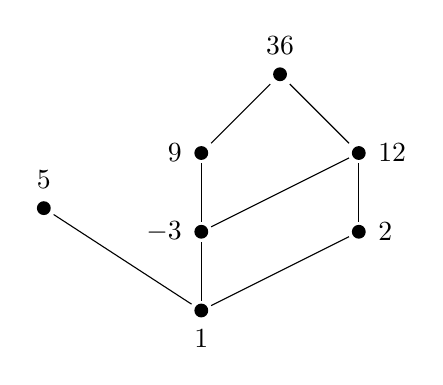
\begin{tikzpicture}
    \fill (9,4) circle[radius=2.5pt] node[label=above:$ {36}$] (36) {};
    
    \fill (8,3) circle[radius=2.5pt] node[label=left:$ {9}$] (9) {};
    \fill (10,3) circle[radius=2.5pt] node[label=right:$ {12}$] (12) {};
    
    \fill (6,2.3) circle[radius=2.5pt] node[label=above:$ {5}$] (5) {};
    \fill (8,2) circle[radius=2.5pt] node[label=left:$ {-3}$] (-3) {};
    \fill (10,2) circle[radius=2.5pt] node[label=right:$ {2}$] (2) {};
    
    \fill (8,1) circle[radius=2.5pt] node[label=below:$ {1}$] (1) {};
    
    \draw (1) -- (5);
    \draw (1) -- (-3);
    \draw (1) -- (2);
    \draw (-3) -- (9);
    \draw (-3) -- (12);
    \draw (2) -- (12);
    \draw (9) -- (36);
    \draw (12) -- (36);

\end{tikzpicture}

\begin{enumerate}[(a)]
    \item 
    No, 5 and 36 are both maximal. There is no maximum element.
    \item
    Yes, 1 is the minimum element
    \item
    No, 1 and 3 are both lower bounds of \{9, 12\}
    \item
    Yes, 12 and 36 are upper bounds
    \item
    Yes, it is.
\end{enumerate}


\end{solution}\probheadernum{4}


If graph $A = K_8$, graph $B = K_{10}$, and graphs $A$ and $B$ share exactly 5 vertices, then how many edges are in $A \cup B$?

\begin{enumerate} [(a)]
    \item 26
    \item 36
    \item 63
    \item 68
    \item 73
\end{enumerate}

\begin{solution}
(c)

Using the Principle of Inclusion/Exclusion, we are able to compute the number of edges in the union of the two graphs:

$|E_{A \cup B}| = |E_A| + |E_B| - |E_{A \cap B}|$

Since each of graphs A, B, and $A \cap B$ are complete graphs, then the number of edges in each individual graph on the RHS is equal to the number of vertices choose 2, or in other words, $\frac{v \cdot (v - 1)}{2}$ where v equals the number of vertices in each graph. Therefore, $|E_{A \cup B}| = \frac{8 \cdot 7}{2} + \frac{10 \cdot 9}{2} - \frac{5 \cdot 4}{2} = 28 + 45 - 10 = 63$
\end{solution}

\newpage
\begin{enumerate}[(a)]
	\item  26
    
	\item  36
    
	\item  63
    
	\item  68
    
	\item  73

\end{enumerate}
\begin{solution}

(c)

Using the Principle of Inclusion/Exclusion, we are able to compute the number of edges in the union of the two graphs:

$|E_{A \cup B}| = |E_A| + |E_B| - |E_{A \cap B}|$

Since each of graphs A, B, and $A \cap B$ are complete graphs, then the number of edges in each individual graph on the RHS is equal to the number of vertices choose 2, or in other words, $\frac{v \cdot (v - 1)}{2}$ where v equals the number of vertices in each graph. Therefore, $|E_{A \cup B}| = \frac{8 \cdot 7}{2} + \frac{10 \cdot 9}{2} - \frac{5 \cdot 4}{2} = 28 + 45 - 10 = 63$

\end{solution}\probheadernum{4}


Find the number of the non-negative integer solutions to the equation 
$$a + b + c + d + e + f + g = 47$$

\begin{enumerate} [(a)]
    \item $\binom{53}{6}$
    \item $\binom{54}{7}$
    \item $\frac{47!}{40!}$
    \item $\binom{47}{7}$
    \item $47!$
\end{enumerate}


\begin{solution}
(a)

This is a Stars 'n Bars. We have 7 variables, so 6 bars, and 47 stars, thus resulting in answer choice (a). 
\end{solution}
\begin{enumerate}[(a)]
	\item  $\binom{53}{6}$
    
	\item  $\binom{54}{7}$
    
	\item  $\frac{47!}{40!}$
    
	\item  $\binom{47}{7}$
    
	\item  $47!$

\end{enumerate}
\begin{solution}

(a)

This is a Stars 'n Bars. We have 7 variables, so 6 bars, and 47 stars, thus resulting in answer choice (a). 

\end{solution}\probheadernum{4}


Which of the following posets have a greatest element?
\begin{enumerate}[(a)]
	\item  
    $(S, |)$, where $S = \{2, 3, 5, 10\}$.
    
	\item  
    $(S, |)$, where $S = \{2, 3, 5, 6, 12, 20, 60 \}$.
    
	\item  
    $(S, \leq)$, where $S = \{x \in \Q: 0 \leq x^2 \leq 3\}$.
    
	\item  
    $(\mathcal{P}(\R), \subseteq)$

\end{enumerate}
\begin{solution}

(b), (d).

(a) has two maximal elements (3,10) and thus has no greatest element.

(b) has only one maximal element, so it has a greatest element.

(c) has no maximal element as $\sqrt{3}$ is not a rational number, so it does not have a greatest element.

(d) has one maximal element which is $\R$, so it has a greatest element.


\end{solution}\probheadernum{4}


Given sets $A$, $B$, and $C$ such that $|A| = 3, |B| = 6$, and $|C| = 8$, which of the following \textbf{could be true}? Select all that apply.


\begin{enumerate} [(a)]
    \item $|A \cap C| = 8$
    \item $|(C - B) \times A| = 9$
    \item $B$ is the power set of $A$
    \item $C$ is the power set of $A$
    \item $\left( (A \times B) \cap C \neq \varnothing \right) \wedge \left( A \cap C \neq \varnothing \right)$
\end{enumerate}


\begin{solution}
(b), (d), (e)

\begin{enumerate}[(a)]
\end{enumerate}
\begin{solution}

(b), (d), (e)

\begin{enumerate}[(a)]
    \item $A \cap C = 8$ cannot be true since the maximum number of terms in the intersection of two sets is equal to the minimum cardinality of the two sets which in this case is 3.
    \item
    Secondly, if $|(C - B) \times A| = 9$ is true, then $|(C - B)| = 3$ since $|A| = 3$. This can be true if 5 of the 6 elements of set B are included in set C meaning that $|(C - B)| = 8 - 5 = 3$. This means that answer (b) can be correct.
    \item
    $B = P(A)$ is not possible since $6 \neq 2^3$.
    \item
    $C = P(A)$ could be true since the number of terms in a power set of a set is $2^n$ and $8 = 2^3$ therefore it is possible. So answer (d) could be correct.
    \item
    When considering $(A \times B)  \cap C  \neq \varnothing \wedge A \cap C \neq \varnothing$, let us consider the following: $\{1, (1,2)\} \subset A, \{2\} \subset b$, and $\{(1,2)\} \subset C$. This would mean that $\{(1,2)\} \subset (A \times B)$ and therefore that $\{(1,2)\} \subset (A \times B) \cap C$. Now considering the second part of the statement, $\{(1,2)\} \subset A$ meaning that $\{(1,2)\} \subset A \cap C$. With these two examples together, we have shown that answer (e) can be correct.
\end{enumerate}
    


\end{solution}\probheadernum{4}
\\
    Which of the following relations on $\{A, B, C, D, E\}$ is a function?
    
    \begin{enumerate} [a)]
        \item 
        \begin{tikzpicture}[->,>=stealth',shorten >=1pt,auto,node distance=1.8cm,
                            semithick]
          \tikzstyle{every state}=[fill=black,draw=none,text=white]
        
          \node[state]         (A)                    {A};
          \node[state]         (B) [above right of=A] {B};
          \node[state]         (D) [below right of=A] {D};
          \node[state]         (C) [below right of=B] {C};
          \node[state]         (E) [below right of=C] {E};
        
          \path 
                (A) edge [loop left] (A)
                (B) edge [loop above] (B)
                (C) edge [loop above] (C)
                (E) edge [loop above] (E)
                (B) edge [bend right=10] (A)
                (A) edge [bend right=10] (B)
                (B) edge [bend right=10] (D)
                (D) edge [bend right=10] (B)
                (A) edge [bend right=10] (D)
                (D) edge [bend right=10] (A)
                (C) edge [bend right=10] (E)
                (E) edge [bend right=10] (C)
                ;
        \end{tikzpicture}
        \item 
        \begin{tikzpicture}[->,>=stealth',shorten >=1pt,auto,node distance=1.8cm,
                            semithick]
          \tikzstyle{every state}=[fill=black,draw=none,text=white]
        
          \node[state]         (A)                    {A};
          \node[state]         (B) [above right of=A] {B};
          \node[state]         (D) [below right of=A] {D};
          \node[state]         (C) [below right of=B] {C};
          \node[state]         (E) [below right of=C] {E};
        
          \path 
                (A) edge [bend right=10] (C)
                (B) edge [bend right=10] (D)
                (C) edge [bend right=10] (E)
                (D) edge [bend right=10] (A)
                (B) edge [bend right=10] (C)
                ;
        \end{tikzpicture}
        \item 
        \begin{tikzpicture}[->,>=stealth',shorten >=1pt,auto,node distance=1.8cm,
                            semithick]
          \tikzstyle{every state}=[fill=black,draw=none,text=white]
        
          \node[state]         (A)                    {A};
          \node[state]         (B) [above right of=A] {B};
          \node[state]         (D) [below right of=A] {D};
          \node[state]         (C) [below right of=B] {C};
          \node[state]         (E) [below right of=C] {E};
        
          \path 
                (A) edge [bend right=10] (C)
                (B) edge [bend right=10] (D)
                (C) edge [bend right=10] (E)
                (D) edge [bend right=10] (A)
                (B) edge [bend right=10] (C)
                (B) edge [loop above] (B)
                ;
        \end{tikzpicture}
        \item 
        \begin{tikzpicture}[->,>=stealth',shorten >=1pt,auto,node distance=1.8cm,
                            semithick]
          \tikzstyle{every state}=[fill=black,draw=none,text=white]
        
          \node[state]         (A)                    {A};
          \node[state]         (B) [above right of=A] {B};
          \node[state]         (D) [below right of=A] {D};
          \node[state]         (C) [below right of=B] {C};
          \node[state]         (E) [below right of=C] {E};
        
          \path 
                (A) edge [bend right=10] (C)
                (B) edge [bend right=10] (D)
                (C) edge [bend right=10] (E)
                (D) edge [bend right=10] (A)
                (E) edge [bend right=10] (C)
                ;
        \end{tikzpicture}
        \item 
        \begin{tikzpicture}[->,>=stealth',shorten >=1pt,auto,node distance=1.8cm,
                            semithick]
          \tikzstyle{every state}=[fill=black,draw=none,text=white]
        
          \node[state]         (A)                    {A};
          \node[state]         (B) [above right of=A] {B};
          \node[state]         (D) [below right of=A] {D};
          \node[state]         (C) [below right of=B] {C};
          \node[state]         (E) [below right of=C] {E};
        
          \path 
                (A) edge [bend right=10] (C)
                (B) edge [bend right=10] (D)
                (C) edge [bend right=10] (E)
                (D) edge [bend right=10] (A)
                (E) edge [bend right=10] (C)
                (C) edge [bend right=10] (B)
                ;
        \end{tikzpicture}
    \end{enumerate}
    \begin{solution}
        (d)  To be a function, a relation must have each element map to exactly 1 element.
    \end{solution}
    


%Atreya 2\begin{enumerate}[(a)]
	\item  
        \begin{tikzpicture}[->,>=stealth',shorten >=1pt,auto,node distance=1.8cm,
                            semithick]
          \tikzstyle{every state}=[fill=black,draw=none,text=white]
        
          \node[state]         (A)                    {A};
          \node[state]         (B) [above right of=A] {B};
          \node[state]         (D) [below right of=A] {D};
          \node[state]         (C) [below right of=B] {C};
          \node[state]         (E) [below right of=C] {E};
        
          \path 
                (A) edge [loop left] (A)
                (B) edge [loop above] (B)
                (C) edge [loop above] (C)
                (E) edge [loop above] (E)
                (B) edge [bend right=10] (A)
                (A) edge [bend right=10] (B)
                (B) edge [bend right=10] (D)
                (D) edge [bend right=10] (B)
                (A) edge [bend right=10] (D)
                (D) edge [bend right=10] (A)
                (C) edge [bend right=10] (E)
                (E) edge [bend right=10] (C)
                ;
        \end{tikzpicture}
        
	\item  
        \begin{tikzpicture}[->,>=stealth',shorten >=1pt,auto,node distance=1.8cm,
                            semithick]
          \tikzstyle{every state}=[fill=black,draw=none,text=white]
        
          \node[state]         (A)                    {A};
          \node[state]         (B) [above right of=A] {B};
          \node[state]         (D) [below right of=A] {D};
          \node[state]         (C) [below right of=B] {C};
          \node[state]         (E) [below right of=C] {E};
        
          \path 
                (A) edge [bend right=10] (C)
                (B) edge [bend right=10] (D)
                (C) edge [bend right=10] (E)
                (D) edge [bend right=10] (A)
                (B) edge [bend right=10] (C)
                ;
        \end{tikzpicture}
        
	\item  
        \begin{tikzpicture}[->,>=stealth',shorten >=1pt,auto,node distance=1.8cm,
                            semithick]
          \tikzstyle{every state}=[fill=black,draw=none,text=white]
        
          \node[state]         (A)                    {A};
          \node[state]         (B) [above right of=A] {B};
          \node[state]         (D) [below right of=A] {D};
          \node[state]         (C) [below right of=B] {C};
          \node[state]         (E) [below right of=C] {E};
        
          \path 
                (A) edge [bend right=10] (C)
                (B) edge [bend right=10] (D)
                (C) edge [bend right=10] (E)
                (D) edge [bend right=10] (A)
                (B) edge [bend right=10] (C)
                (B) edge [loop above] (B)
                ;
        \end{tikzpicture}
        
	\item  
        \begin{tikzpicture}[->,>=stealth',shorten >=1pt,auto,node distance=1.8cm,
                            semithick]
          \tikzstyle{every state}=[fill=black,draw=none,text=white]
        
          \node[state]         (A)                    {A};
          \node[state]         (B) [above right of=A] {B};
          \node[state]         (D) [below right of=A] {D};
          \node[state]         (C) [below right of=B] {C};
          \node[state]         (E) [below right of=C] {E};
        
          \path 
                (A) edge [bend right=10] (C)
                (B) edge [bend right=10] (D)
                (C) edge [bend right=10] (E)
                (D) edge [bend right=10] (A)
                (E) edge [bend right=10] (C)
                ;
        \end{tikzpicture}
        
	\item  
        \begin{tikzpicture}[->,>=stealth',shorten >=1pt,auto,node distance=1.8cm,
                            semithick]
          \tikzstyle{every state}=[fill=black,draw=none,text=white]
        
          \node[state]         (A)                    {A};
          \node[state]         (B) [above right of=A] {B};
          \node[state]         (D) [below right of=A] {D};
          \node[state]         (C) [below right of=B] {C};
          \node[state]         (E) [below right of=C] {E};
        
          \path 
                (A) edge [bend right=10] (C)
                (B) edge [bend right=10] (D)
                (C) edge [bend right=10] (E)
                (D) edge [bend right=10] (A)
                (E) edge [bend right=10] (C)
                (C) edge [bend right=10] (B)
                ;
        \end{tikzpicture}
    
\end{enumerate}
\begin{solution}

        (d)  To be a function, a relation must have each element map to exactly 1 element.
    
\end{solution}\probheadernum{4}
\\
5 people want to play doubles ping-pong. They are going to split up into two pairs, and one of them will referee the game. How many different ways are there to set up the game?

\begin{enumerate}[(a)]
	\item  $\frac{\binom{5}{1} \cdot \binom{4}{2} \cdot \binom{2}{2}}{2!}$

	\item  $\binom{5}{1} \cdot \binom{4}{2} \cdot \binom{2}{2}$

	\item  $\frac{5!}{2! \cdot 2!}$

	\item  $\binom{5}{1} \cdot 2^4$

	\item  $\frac{5!}{4! \cdot 2}$

\end{enumerate}
\begin{solution}

(a)\\
choose the referee $\binom{5}{1}$, then select two players who will be on a team $\binom{4}{2}$ and select the other two remaining who will be on a team $\binom{2}{2}$. Then we divide by $2!$ because we overcount the case we choose AB then CD and the case we choose CD and then AB since they both set up the game the same way.

\end{solution}\probheadernum{4}
\\
In the binomial expansion of $(x^3 - 1/{x^4})^{12}$, what is the coefficient of the $x^{15}$?
\begin{enumerate}[a)]
    \item $-\binom{12}{9}$
    \item $\binom{12}{9}$
    \item $\binom{12}{6}$
    \item $-\binom{12}{6}$
    \item $0$
\end{enumerate}
\begin{solution}
(a)\\
Use the binomial theorem to express as\\  $\sum_{a=0}^{12}\binom {12}a(x^3)^a \cdot (-x^{-4})^{12-a}=\sum_{a=0}^{12}\binom {12}ax^{3a} \cdot (-1)^{12-a}x^{-48+4a}=\sum_{a=0}^{12}\binom {12}ax^{7a-48} \cdot (-1)^{12-a}$. when exponent $15 = 7a - 48$, we have $a = 9$. Therefore the coefficient is $\binom{12}{9} \cdot (-1)^3$
\end{solution}
\begin{enumerate}[(a)]
	\item  $-\binom{12}{9}$
    
	\item  $\binom{12}{9}$
    
	\item  $\binom{12}{6}$
    
	\item  $-\binom{12}{6}$
    
	\item  $0$

\end{enumerate}
\begin{solution}

(a)\\
Use the binomial theorem to express as\\  $\sum_{a=0}^{12}\binom {12}a(x^3)^a \cdot (-x^{-4})^{12-a}=\sum_{a=0}^{12}\binom {12}ax^{3a} \cdot (-1)^{12-a}x^{-48+4a}=\sum_{a=0}^{12}\binom {12}ax^{7a-48} \cdot (-1)^{12-a}$. when exponent $15 = 7a - 48$, we have $a = 9$. Therefore the coefficient is $\binom{12}{9} \cdot (-1)^3$

\end{solution}\probheadernum{4}
\\
Let relation $R$ be $a$ relates to $b$ iff $a$ and $b$ have the same number of digits that are 5 (for example $(45, 500)\in R$ and $(55, 550)\in R$).  Let the domain of $R$ be the set of integers from 1 to 1000. What is the cardinality of the equivalence class of 55.
\begin{enumerate}[a)]
    \item 27
    \item 28
    \item 29
    \item 30
    \item 729
\end{enumerate}
\begin{solution}
(a) \\
We can treat the number 0 through 999 as 3-digit numbers with leading 0s if you need them (e.g. 7 = 007).  55 does not relate to 0 or 1000, so we don't need to worry about those boundary issues.  We need to consider how to assign the 3 digits to get exactly two 5s.  We select which two to be 5s $\binom 32$, and then select what digit other than 5 the other digit is (9).  Multiplying these, we get $$\binom32\cdot 9=27$
\end{solution}

\begin{enumerate}[(a)]
	\item  27
    
	\item  28
    
	\item  29
    
	\item  30
    
	\item  729

\end{enumerate}
\begin{solution}

(a) \\
We can treat the number 0 through 999 as 3-digit numbers with leading 0s if you need them (e.g. 7 = 007).  55 does not relate to 0 or 1000, so we don't need to worry about those boundary issues.  We need to consider how to assign the 3 digits to get exactly two 5s.  We select which two to be 5s $\binom 32$, and then select what digit other than 5 the other digit is (9).  Multiplying these, we get $$\binom32\cdot 9=27$

\end{solution}\probheadernum{4}
\\
Out in 3D space, we have coordinates in the $x, y,$ and $z$ dimension. We have a spaceship that can only move in three possible directions, one coordinate unit at a time: towards \textbf{positive} $x, y,$ or $z$. 

In other words, if we are at location $(x,y,z)$, there are 3 locations we can travel to next:
\begin{itemize}
    \item $(x+1,y,z)$
    \item $(x,y+1,z)$
    \item $(x,y,z+1)$
\end{itemize}

It costs 1 gallon of fuel to move 1 coordinate unit distance. Our spaceship starts at the origin (0,0,0) and we must use up all 25 gallons of fuel that our ship has.  How many possible end destinations does our spaceship have? \\\\
For example, $(10,7,8)$ is one possible destination, but $(0,0,1)$ is not possible, because that would only use up 1 gallon of fuel (and we are not able to travel in negative directions to waste the fuel).
\begin{enumerate}[a)]
    \item $\binom{27}{2}$
    \item $\binom{25}{3}$
    \item $\frac{25!}{22!}$
    \item $\frac{27!}{25!}$
    \item $3^{25}$
\end{enumerate}
\begin{solution}
(a) \\
The order we make our moves doesn't matter, only where we end up, so we are just asking how many non-negative integer $(x,y,z)$ coordinates have $x+y+z=25$.  This is a stars and bars problem, with 25 stars and 3 categories (towards x towards y towards z), so 2 bars.   $\binom{27}{2}$. 
\end{solution}

\begin{enumerate}[(a)]
	\item  $(x+1,y,z)$
    
	\item  $(x,y+1,z)$
    
	\item  $(x,y,z+1)$
\end{itemize}

It costs 1 gallon of fuel to move 1 coordinate unit distance. Our spaceship starts at the origin (0,0,0) and we must use up all 25 gallons of fuel that our ship has.  How many possible end destinations does our spaceship have? \\\\
For example, $(10,7,8)$ is one possible destination, but $(0,0,1)$ is not possible, because that would only use up 1 gallon of fuel (and we are not able to travel in negative directions to waste the fuel).
\begin{enumerate}[a)]
    
	\item  $\binom{27}{2}$
    
	\item  $\binom{25}{3}$
    
	\item  $\frac{25!}{22!}$
    
	\item  $\frac{27!}{25!}$
    
	\item  $3^{25}$

\end{enumerate}
\begin{solution}

(a) \\
The order we make our moves doesn't matter, only where we end up, so we are just asking how many non-negative integer $(x,y,z)$ coordinates have $x+y+z=25$.  This is a stars and bars problem, with 25 stars and 3 categories (towards x towards y towards z), so 2 bars.   $\binom{27}{2}$. 

\end{solution}\probheadernum{4}
\\
What is the big-$\Theta$ runtime of the following algorithm, based on the number of print statements?

\begin{algorithm}[H]
    \SetKwFunction{goodLuck}{goodLuck}{}
    \SetKwFunction{Print}{print}
    \SetKwProg{Fn}{procedure}{\string:}{}
    \SetKwFor{For}{for}{do}{}
    \SetKwFor{If}{if}{then}{}
    \SetKwInOut{Input}{input}
    \DontPrintSemicolon
    \Input{$n$ is an integer, $x$ an integer}
    \BlankLine
    \Fn{\goodLuck{n, x}}{
        \If {$n = 1$} {
            \KwRet{}
        }
        a := \goodLuck{$n/2$, $x$}\;
        b := \goodLuck{$n/2$, $x+1$}\;
        c := \goodLuck{$n/2$, $x+2$}\;
        \For{$j\leftarrow 1$ \KwTo n}{
            \Print{``Good Luck!''}
        }
         \KwRet{a + b + c}
     }
     \caption{goodLuck}
\end{algorithm}

\begin{enumerate} [a)]
    \item $\Theta (n^{\log_2 3})$ 
    \item $\Theta (n)$
    \item $\Theta (n \log_2 3) $
    \item $\Theta (n^2)$
    \item $\Theta (n^3)$
\end{enumerate}

\begin{solution}
(a) \\
$T(n) = 3T(n/2) + n$. Using master theorem, $a = 3, b=2, d=1$, so we get the runtime is $\Theta (n^{\log_2 3})$.
\end{solution}

%%%%%%%%%%%%%%%%%%%%%%%%%%%%%%%%%%%%%%%%%%%%%
%%% 		PART A2 BEGINS HERE			  %%%
%%%%%%%%%%%%%%%%%%%%%%%%%%%%%%%%%%%%%%%%%%%%%
\newpage\begin{enumerate}[(a)]
	\item  $\Theta (n^{\log_2 3})$ 
    
	\item  $\Theta (n)$
    
	\item  $\Theta (n \log_2 3) $
    
	\item  $\Theta (n^2)$
    
	\item  $\Theta (n^3)$

\end{enumerate}
\begin{solution}

(a) \\
$T(n) = 3T(n/2) + n$. Using master theorem, $a = 3, b=2, d=1$, so we get the runtime is $\Theta (n^{\log_2 3})$.

\end{solution}\probheadernum{4}
\\
Let 
\begin{align*}
    a \equiv 3 \pmod{12}\\
    b \equiv 2 \pmod{15}\\
    c \equiv 1 \pmod{4}
\end{align*}
Which of these must be true:
\begin{enumerate}[(a)]
	\item  $2a \equiv c \pmod{4}$

	\item  $a + c \equiv 0 \pmod{4}$

	\item  $a + b \equiv 2 \pmod{3}$

	\item  $3c \equiv 11 \pmod{4}$

	\item  $a - b \equiv 1 \pmod{15}$

\end{enumerate}
\begin{solution}

b, c, d\\
Because $a\equiv 3\pmod {12}$, we also know $a\equiv 3\pmod 4$ and $a\equiv 3\pmod 3$.  Similarly, we know $b\equiv 2\pmod 3$ and $b\equiv 2\pmod 5$.\\
(a) $2a\equiv 2\not\equiv1\equiv c\pmod 4$\\
(b) $a+c\equiv 3+1\equiv 0\pmod 4$\\
(c) $a+b\equiv 3+2\equiv 5\equiv 2\pmod 3$\\
(d) $3c\equiv 3\equiv 11\pmod 4$\\
(e) We don't know what $a$ is mod 15, so we don't know what $a-b$ is mod 15.  For example, perhaps $a=15\equiv 3\pmod {12}$ as needed.  This would make $a-b= 15-2\equiv 13\pmod {15}$  

\end{solution}\probheadernum{4}
\\
title page question

\begin{enumerate}[(a)]
\end{enumerate}
\begin{solution}
uestion


\end{solution}\probheadernum{4}

% Team 3, Question 1

Brian is shopping for ice cream, and the grocery store has 6 pints left, each of a different flavor. He doesn't want to come back empty-handed, so he buys at least one pint. In how many ways can he buy his ice cream?

\begin{enumerate}[(a)]
	\item  $2^6-1$

	\item  $2^6$

	\item  $\binom{7}{6}-1$

	\item  $\binom{7}{6}$

	\item  $6$

\end{enumerate}
\begin{solution}

(a)\\
There are $2$ options for each flavor of ice cream (in/out) and there are $6$ flavors of ice cream. However, we are overcounting the scenario of all $6$ flavors being out since Brian has to buy at least $1$ pint of ice cream, so we subtract $1$.

\end{solution}\probheadernum{4}
\\
% Team 4, Question 5
% TODO: Tweak to make balanced case??
What is the runtime complexity of the following algorithm:
% See: http://mirror.hmc.edu/ctan/macros/latex/contrib/algorithm2e/doc/algorithm2e.pdf
\begin{algorithm}[H]
    \SetKwFunction{f}{badSearch}{}
    \SetKwFunction{Print}{print}
    \SetKwProg{Fn}{procedure}{\string:}{}
    \SetKwFor{For}{for}{}{}
    \SetKwFor{While}{while}{}{}
    \SetKwFor{If}{if}{then}{}
    \SetKwInOut{Input}{input}
    \DontPrintSemicolon
    \Input{$n$ an integer}
    \BlankLine
    %REMEMBER: \; ends a line!
    \Fn{\f{n}}{
        \If{$n=1$} \KwRet{}
        \f{$n/3$}\; 
        \f{$n/3$}\; 
        \For{$i := 1$ \KwTo $n$}{
            \For{$j := 1$ \KwTo $10$}{
                \Print{``Hello, I am lost.''}\;
            }
         }
        \f{$n/3$}\; 
        \Print{``Nevermind, I got it.''}\;
        \KwRet{}
     }
     \caption{A bad search algorithm}
\end{algorithm}
\begin{enumerate}[(a)]
	\item  $\Theta(n)$

	\item  $\Theta(n^{\log_3(2)})$

	\item  $\Theta(n^2)$

	\item  $\Theta(n\log(n))$

	\item  $\Theta(n^{\log_2(3)})$

\end{enumerate}
\begin{solution}

(c)\\
The recurrence is $T(n)=2T(n/3)+O(n^2)$. Since $\frac{2}{3^2}<1$, by the Master Theorem this algorithm is $\Theta(n^2)$.

\end{solution}\probheadernum{4}
\\
% Additional, Question 1
Suppose we want to find a solution to the following system of linear congruences:
\begin{center}
$x \equiv 2 \mod{7}$\\
$x \equiv 6 \mod{10}$\\
$x \equiv 11 \mod{13}$\\
\end{center}
Which of the following terms must be computed when solving for $x$ using the Chinese Remainder Theorem
\begin{enumerate}[(a)]
	\item  $(6 \cdot 11)^{-1} \mod{7}$

	\item  $(7 \cdot 6 \cdot 13)^{-1} \mod{10}$

	\item  $(7 \cdot 10)^{-1} \mod{13}$

	\item  $2 \cdot 6 \cdot 11$

	\item  $7 \cdot 10 \cdot 13$

\end{enumerate}
\begin{solution}

(c)(e)\\
Using the Chinese Remainder Theorem, we can compute $x$ as:\\
\scalebox{0.7}{
$x \equiv \left(2 \cdot (10 \cdot 13) \cdot [(10 \cdot 13)^{-1} \mod{7}] + 6 \cdot (7 \cdot 13) \cdot [(7 \cdot 13)^{-1} \mod{10}] + 11 \cdot (7 \cdot 10) \cdot [(7 \cdot 10)^{-1} \mod{13}] \right) \mod{7 \cdot 10 \cdot 13}$.
}\\
We need to calculate the inverses of the products of two moduli mod the other modulus (c), as well as the product of all the moduli (e).

\end{solution}\probheadernum{4}
\\
% Additional, Question 4
Let $A$, $B$, and $C$ be three distinct prime numbers such that $A=2B+1$. Which of the following are correct?  

\textit{Note:} Make sure to read each modulus, as they are not all the same.
\begin{enumerate}[(a)]
	\item  $C^{AB}\equiv C^B\pmod{A}$

	\item  $C^{AB}\equiv C^3\pmod{B}$

	\item  $B^{-1}\equiv -2\pmod{A}$

	\item  $A^{-1}\equiv 1\pmod{B}$

\end{enumerate}
\begin{solution}

(a)(b)(c)(d)
\begin{enumerate}[(a)]
\item Since $A$ is prime and $C$ is not divisible by $A$, we have $C^{A}\equiv C\pmod{A}$ by Fermat’s Little Theorem. Then $C^{AB}=(C^{A})^B\equiv (C)^B\pmod{A}$.
\item Similarly, we know that $C^{B}\equiv C\pmod{B}$ and $C^{AB}\equiv C^A\pmod{B}$, which can be turned into $C^A=C^{2B+1}=(C^B)^2\cdot C =(C)^2\cdot C\equiv C^3\pmod{B}$.
\item It is sufficient to verify whether $B(-2)\equiv1\pmod{A}$. Indeed, $B(-2)=-2B\equiv A-2B=(2B+1)-2B\equiv1\pmod{A}$.
\item Since $A=2B+1$, we get that $A\equiv 1\pmod{B}$. Then $A^{-1}\equiv1^{-1}\equiv1\pmod{B}$.
\end{enumerate}

\end{solution}\probheadernum{4}


Four people are standing in a circle as shown. Each person is given a T-shirt to wear.  The shirts come in 3 different colors, and any two people next to each other cannot wear the same color shirt. How many ways are there to give T-shirts to the four people?
\vspace{0.1in}

\begin{minipage}{.3\textwidth}
\begin{enumerate}[(a)]
	\item  15
    
	\item  18
    
	\item  24
    
	\item  36
    
	\item  40

\end{enumerate}
\begin{solution}

% Team 3.2

(b)

We can start with person A, and A has 3 choices. The two people next to A are B and D, and they can be in the same color or different colors.

\begin{enumerate}
    \item If B and D are in the same color, there are 2 ways to color B and D, and there are also 2 ways to color C, since B and D are C's neighbors and they are in the same color. For this case, there are $3\cdot 2\cdot 2 = 12$ ways.
    \item If B and D are in different colors, then there are 2 ways to color B, and 1 ways to color D, since D has to be different with both A and B. Since B and D are C's neighbors and they have different colors, there is 1 way to give C colors. For this case, there are $3\cdot 2\cdot 1\cdot1 = 6$ ways.
\end{enumerate}
The two cases sum up to 18.

\end{solution}\probheadernum{4}


% If an office building has 47 floors with 30 offices per floor, how many ways are there to give three people offices (if they are all empty) if offices on the same floor are not distinguishable. People are considered distinguishable from each other.

% \begin{enumerate}[(a)]
	\item {$\binom{30\cdot47}{3}$}
% 
	\item {$47^3$}
% 
	\item {$\frac{47!}{30!3!}$}
% 
	\item {$\frac{47!}{33!}$}
% 
	\item {$P(47,3)$}
% 
\end{enumerate}
\begin{solution}

% (b)
% % Team 3.5

% Since each office on a given floor is the same, and since there are enough offices on each floor for everyone to be on the same floor, this is the same as choosing which floor each person is on. Since there are $47$ floors/options for each of the three people, there are $47^3$ ways to assign floors to these three employees. 
% 
\end{solution}\probheadernum{4}
\\
% Brainstorm 4.7
Consider two fair, six-sided dice with non-standard faces. One die is red and the other is blue. The red die has faces 1, 2, 2, 3, 3, 4, and the blue die has faces 2, 2, 4, 6, 6, 8.  Let $X$ be the sum of the faces when the dice are rolled. What is $p(X \geq 10)$?
%The red dice has the sides 1, 2, 2, 3, 3, 4. The blue dice has the sides 2, 2 ,4, , 8, 8. Both dices are standard six-sided dice so that each face shows up equally likely. What is $p(X \geq 10)$?
\begin{enumerate}[(a)]
	\item  $\dfrac{1}{4}$ %There are 4 unique faces per dice, so 16 total. 4 sums are geq 10.

	\item  $\dfrac{1}{9}$ %p(X=10)

	\item  $\dfrac{3}{10}$ %there are 10 unique sums, 3 of which are geq than 10

	\item  $\dfrac{7}{36}$ %right answer

	\item  $\dfrac{10}{36}$ %10 is in the problem and 36 is 6^2

\end{enumerate}
\begin{solution}

(d)\\
There are 7 possible roll combinations that result in a sum greater or equal to than 10: $\{(2,8), (2,8), (4,6), (4,6), (3,8), (3,8), (4,8)\}$. There are 36 total roll combinations, so the probability is $\frac{7}{36}$.

\end{solution}\probheadernum{4}


How many permutations of the string ``ABCDEFGHIJKLMNOPQRSTUVWXYZ" contain the substrings ``HAVE" and ``FUN"?
Substrings must appear exactly as written. 

\textit{e.g.,} LCQOPGRK\underline{\textbf{FUN}}TYDIWS\underline{\textbf{HAVE}}ZXMJB is a valid substring.
%where the letters in each substring are consective and in order. 
%with the designated letters consecutive and in order.
\begin{enumerate}[(a)]
	\item  $\dfrac{26!}{4!3!}$
    
	\item  $\dfrac{26!}{20!}$
    
	\item  20!
    
	\item  $2 \cdot 20!$
    
	\item  $21!$

\end{enumerate}
\begin{solution}

% Team 2

(e)

Since both ``HAVE" and ``FUN" are substrings and each letter only appears once in the permutation of the string, we can consider each of those substrings as a single unit. Now, we consider all permutations of $26 - 3 - 4 + 2= 21$ items, of which there are $21!$ of them. 

\end{solution}\probheadernum{4}
\\
% Brainstorm 4.4
Balls numbered from 1 to 203 are placed inside a box. You randomly draw six balls from the box one at a time without replacement. What is the probability that the numbers on the balls are drawn in decreasing order? An example of this would be first drawing the ball with 203, then 200, 199, 150, 100, 40. \\
In the answer choices, $P$ refers to permutations.
\begin{enumerate}[(a)]
	\item  $\dfrac{1}{6!}$

	\item  $\dfrac{1}{P(203, 6)}$

	\item  $\dfrac{6!}{P(203, 6)}$

	\item  $\dfrac{203}{P(203, 6)}$

	\item  $\dfrac{1}{\binom{203}6}$


\end{enumerate}
\begin{solution}

(a)\\
We can think of this as first picking the 6 balls. There are only 6! possible ways to order the balls by the numbers on them, and only one of these orders is decreasing.

\end{solution}\probheadernum{4}


Let $a,b,n \in \mathbb{Z}^+$. Given $a+b = n$, which of the following are true?
\begin{enumerate}[(a)]
	\item {$\dbinom{n}{a} = \dbinom{n}{b}$}

	\item {$P(n,a) = P(n,b)$}

	\item {$\dbinom{n-1}{a-1} + \dbinom{n-1}{a} = \dbinom{n}{a}$}

	\item {$\dfrac{P(n,b)}{b!} = \dfrac{P(n,a)}{a!}$}

	\item {$\dbinom{n}{b}\dbinom{n-b}{a} = \dfrac{n!}{a!b!}$}


\end{enumerate}
\begin{solution}

% Team 3.MC.2
(a),(c),(d), (e)\\
(a):$$ \chyz{n}{a} = \frac{n!}{a!(n-a)!} = \frac{n!}{(n-b)!b!}= \chyz{n}{b}$$
(b): Take $a=1,b=2,n=m$ then $P(n,a) = 3, P(n,b) = 3!=6$ \\
(c): Is a direct result of Bernoulli's Identity.\\
(d): $$\frac{1}{b!}P(n,b) = \frac{1}{b!}\frac{n!}{(n-b)!} = \frac{1}{(n-a)!}\frac{n!}{a!} = \frac{1}{a!}\frac{n}{(n-a)!} = \frac{1}{a!}P(n,a)$$
(e): $$\chyz{n}{b}\chyz{n-b}{a} = \chyz{n}{b} = \frac{n!}{(n-b)!b!} = \frac{n!}{a!b!}$$

\end{solution}\probheadernum{4}


Which of the following are equivalent to $\binom{7}{3}$?
\begin{enumerate}[(a)]
	\item  The number of bit strings of length seven that contain exactly four 0s.
    
	\item  The number of ways to distribute 3 identical candy bars to 5 children.
    
	\item  The number of ways to assign rankings of 1st, 2nd, and 3rd to a group of seven competitors.
    
	\item  The number of possible outcomes that contain at least three heads if a coin is flipped seven times.
    
	\item  The number of possible outcomes that contain one more head than tail if a coin is flipped seven times.

\end{enumerate}
\begin{solution}

% Team 2.3
(a), (b), (e) \\
(a) is correct because this is equal to the number of bit strings of length seven that contain exactly three 1s. (Also, C(7,3) = C(7,4).) \\
(b) can be found with the stars and bars method. There are 3 stars (number of candy bars) and 4 bars (number of children minus one). Then, we have C(stars + bars, stars), which will give us C(7,3). \\
(c) is incorrect because this would be choosing ordered arrangements. \\
(d) is incorrect because the number of possible outcomes that contain \textbf{at least} three heads is equal to C(7,3) + C(7,4) + C(7,5) + C(7,6) + C(7,7). \\
(e) is correct because the only way this can happen is if there are four heads and three tails, which would give us C(7,3).

\end{solution}\probheadernum{4}


What is the constant term in the expansion of $(203x^2+376\frac{1}{x})^{300}$ ?
\begin{enumerate}[{(a)}]
    \item $\binom{300}{100} \cdot 203^{100} \cdot 376^{200}$
    \item $\binom{300}{150} \cdot 203^{150} \cdot 376^{150}$
    \item $203^{100} \cdot 376^{200}$
    \item $203^{150} \cdot 376^{150}$
    \item 0
\end{enumerate}

\begin{solution}
% Hw Team 2
(a) The constant term must have the $x^2$ and $\frac{1}{x}$ cancel out. This happens when there is a $(203x^2)^{100}$ and $(376\frac{1}{x})^{200}$ in the term. Using the binomial expansion formula, the term is $$\binom{300}{100}(203x^2)^{100}(376\frac{1}{x})^{200} = \binom{300}{100}203^{100}376^{200}$$
\end{solution}

\newpage
\begin{enumerate}[(a)]
	\item  $\binom{300}{100} \cdot 203^{100} \cdot 376^{200}$
    
	\item  $\binom{300}{150} \cdot 203^{150} \cdot 376^{150}$
    
	\item  $203^{100} \cdot 376^{200}$
    
	\item  $203^{150} \cdot 376^{150}$
    
	\item  0

\end{enumerate}
\begin{solution}

% Hw Team 2
(a) The constant term must have the $x^2$ and $\frac{1}{x}$ cancel out. This happens when there is a $(203x^2)^{100}$ and $(376\frac{1}{x})^{200}$ in the term. Using the binomial expansion formula, the term is $$\binom{300}{100}(203x^2)^{100}(376\frac{1}{x})^{200} = \binom{300}{100}203^{100}376^{200}$$

\end{solution}\probheadernum{4}


A fair coin is flipped 6 times in a row. Given that the fourth flip is tails, what is the probability that exactly 4 flips come up heads?
\\
\begin{enumerate} [(a)]
    \item $\frac{1}{64}$
    \item $\frac{1}{32}$
    \item $\frac{5}{32}$
    \item $\frac{15}{64}$
    \item $\frac{15}{32}$

\end{enumerate}
\begin{solution}
% Team 3 
c) Because the fourth flip is tails, we are looking for the probability that exactly 4 of the other 5 flips come up heads. This probability can be found using the binomial distribution. We have $n = 5$, and $k = 4$, and $p = 1 - p = 1/2$ (because the coin is fair). Thus, we know that the probability is $\binom{5}{4}(1/2)^4(1/2)^1 = \frac{5}{32}$
\end{solution}

\newpage
\begin{enumerate}[(a)]
	\item  $\frac{1}{64}$
    
	\item  $\frac{1}{32}$
    
	\item  $\frac{5}{32}$
    
	\item  $\frac{15}{64}$
    
	\item  $\frac{15}{32}$


\end{enumerate}
\begin{solution}

% Team 3 
c) Because the fourth flip is tails, we are looking for the probability that exactly 4 of the other 5 flips come up heads. This probability can be found using the binomial distribution. We have $n = 5$, and $k = 4$, and $p = 1 - p = 1/2$ (because the coin is fair). Thus, we know that the probability is $\binom{5}{4}(1/2)^4(1/2)^1 = \frac{5}{32}$

\end{solution}\probheadernum{4}


After repeatedly rolling 2 identical standard dice, you finally notice that a combination has repeated itself. For example, on the second roll, you roll a 1 and a 5, and on the eighth roll, you roll a 5 and a 1.  How many rolls of 2 dice are required to guarantee that some unordered combination has been repeated?  
\begin{enumerate}[{(a)}]
    \item 13
    \item 16
    \item 19
    \item 22
    \item 37
\end{enumerate}
\begin{solution}
% Hw Team 2
% TODO: Team 2 to update solution using stars and bars
(d) There are $\binom{6}{2} = 15$ ways to choose, in no particular order, two distinct numbers, and another 6 ways to choose two repeated numbers. This means there are $15 + 6 = 21$ distinct die rolls and thus there must be 22 rolls of 2 dice in order to guarantee that some combination has been repeated.
\end{solution}

\newpage
\begin{enumerate}[(a)]
	\item  13
    
	\item  16
    
	\item  19
    
	\item  22
    
	\item  37

\end{enumerate}
\begin{solution}

% Hw Team 2
% TODO: Team 2 to update solution using stars and bars
(d) There are $\binom{6}{2} = 15$ ways to choose, in no particular order, two distinct numbers, and another 6 ways to choose two repeated numbers. This means there are $15 + 6 = 21$ distinct die rolls and thus there must be 22 rolls of 2 dice in order to guarantee that some combination has been repeated.

\end{solution}\probheadernum{4}


Six identical prizes are to be given to 12 chefs in a local cook-off. Nevertheless, any individual chef may win anywhere between 0 and 6 prizes, inclusive. How many ways are there to award the chefs the prizes?
\begin{enumerate}[{(a)}]
    \item $\frac{12^6}{6!}$
    \item $12^6$
    \item $\binom{17}{5}$
    \item $\binom{17}{11}$
    \item $\frac{12!}{6!}$
\end{enumerate}
\begin{solution}
% Hw Team 2
(d) By stars n' bars, we see that there are 6 stars and 11 bars. Since the prizes are identical (indistinguishable) then we treat the prizes as stars, and the chefs are distinguishable and are used to calculate bars as $12 - 1 = 11$. Thus, there are $\binom{17}{6} = \binom{17}{11}$ ways to award the chefs the prizes.
\end{solution}

\vspace{2cm}
\begin{enumerate}[(a)]
	\item  $\frac{12^6}{6!}$
    
	\item  $12^6$
    
	\item  $\binom{17}{5}$
    
	\item  $\binom{17}{11}$
    
	\item  $\frac{12!}{6!}$

\end{enumerate}
\begin{solution}

% Hw Team 2
(d) By stars n' bars, we see that there are 6 stars and 11 bars. Since the prizes are identical (indistinguishable) then we treat the prizes as stars, and the chefs are distinguishable and are used to calculate bars as $12 - 1 = 11$. Thus, there are $\binom{17}{6} = \binom{17}{11}$ ways to award the chefs the prizes.

\end{solution}\probheadernum{4}


Computer programs print output to a screen, and sometimes when multiple programs try to print output at the same time, the individual characters get interleaved, while maintaining their original order from within their respective programs. For example, if Program A prints \textbf{abc} and Program B prints \textbf{DEF}, the output may be \textbf{aDbcEF}, but never \textbf{cbaDEF}.

\vspace{0.1in}
If Program 1 prints \textbf{RISHI}, Program 2 prints \textbf{ADAM}, and Program 3 prints\\ \textbf{ELLEN}, how many possible interleavings are there?

\begin{enumerate}[(a)]
	\item  $\frac{14!}{2!2!2!2!}$
    
	\item  $\frac{14!}{8!}$
    
	\item  $\binom{14}{5} \binom{9}{4}$
    
	\item  $\frac{1}{2!2!2!2!} \binom{14}{5} \binom{9}{4}$
    
	\item  $\frac{1}{8!}\binom{14}{5} \binom{9}{4}$

\end{enumerate}
\begin{solution}
 
%Hw Team 2
(c)

There are
\[
    \binom{14}{5} \binom{9}{4}
\]
ways to choose the interleavings, since you first choose the 5 spots for the 5 characters printed by program 1, then choose the 4 spots for the 4 characters printed by program 2. This is because once the spots are chosen, the order of the letters printed by the program is predetermined. 

Note that no overcounting occurs, since the words were chosen carefully so that there is no overlap between the output of the 3 programs. Even though there are two "$i$"s in $rishi$, each $i$ is placed uniquely by the choice of the spots for $rishi$, so no overcounting occurs.

\end{solution}\probheadernum{4}


Which of the following sets are well-ordered under the given ordering?
\begin{enumerate}[(a)]
	\item  ($\mathbb{Q^+} \cup \{0\}$, $<$)

	\item  ($\mathbb{R} \cap \mathbb{N}$, $<$)

	\item  $(\Z^-, <)$

	\item  ($\{\pi, 1, \sqrt{2}, -5\}$, $>$)

	\item  $([0,1], >)$

\end{enumerate}
\begin{solution}

(b), (d)\\
(a) is not well ordered because there is a nonempty subset (e.g. $\mathbb{Q^+}$) that has no least element.\\
(b) is well ordered since this reduces to $\mathbb{N}$ which is well-ordered under $<$.\\
(c) is not well ordered because there is a nonempty subset (e.g. $\mathbb{Z^-}$) that has no least element.\\
(d) is well ordered because every nonempty subset has a least element and a defined ordering.\\
(e) is not well ordered because there is a nonempty subset (e.g. (0, 1)) that has no least element.

\end{solution}